\documentclass{scirep}
\usepackage{amsmath}

\leftheader{Sternův-Gerlachův experiment}
\centerheader{Praktikum IV}
\rightheader{Tomáš Derner}

\begin{document}

    \section*{Úkol}

    \begin{enumerate}

        \item Zkontrolujte vakuum v aparatuře a při dosažení potřebného tlaku zprovozněte detektor atomů draslíku a pícku.
        Sledujte zbytkový proud detektoru a v případě potřeby vyčistěte povrch emisní elektrody doporučeným postupem.
        \item Umístěte detektor do maxima nevychýleného svazku (poloha $\si{7,70}$ indikátoru otáček, $U_x=\SI{583}{mV}$) a sledujte nárůst intenzity svazku s teplotou (použitý rozsah nanoampérmetru je \SI{0,1}{nA}).
        Při dosažení signálu z detektoru cca $\SI{2}{V}$ ohřev pícky zastavte (pro stabilizaci této teploty je nyní potřebné střídavé napětí kolem $\SI{6}{V}$, čerstvá náplň draslíku dává tento signál při cca \SI{160}{\celsius}).
        Překontrolujte, že je napětí z detektoru alespoň a zvolte vhodný rozsah Kanálu 1 (výchozí je $\SI{\pm 5}{V}$).
        \item Pomocí programu Stern-Gerlach proměřte prostorový profil atomového svazku při nulovém magnetickém poli.
        \item Tímtéž programem proměřte profily při magnetizačních proudech $\SI{250}{mA}$ ($B=\SI{0,175}{T}$), $\SI{350}{mA}$ ($B=\SI{0,265}{T}$), $\SI{500}{mA}$ ($B=\SI{0,383}{T}$), $\SI{700}{mA}$ ($B=\SI{0,530}{T}$) a $\SI{1000}{mA}$ ($B=\SI{0,675}{T}$).
        \item Naměřené hodnoty rozštěpení svazku vyneste do grafu závislosti $\frac{\partial B}{\partial z}$ na veličině $q = 3ue - \frac{C}{ue}$ (podle vztahu (15) a obr. 8 studijního textu) a regresí určete hodnotu Bohrova magnetonu.
        Diskutujte přesnost metody a citlivost na vynechání některých hodnot.

    \end{enumerate}

    \section*{Teorie}

    V tomto praktiku se zabýváme Stern-Gerlachovým experimentem, jedním z definujících experimentů kvantové mechaniky.
    Pro měření využíváme aparaturu od firmy PHYWE Gottingen a vakuovou soustavu od firmy VAKUUM Praha.

    Aparatura sestává z pícky, která slouží jako zdroj atomů draslíku, které jsou v tomto experimentu použité namísto stříbra, magnetického analyzátoru a Langmuirova – Taylorova detektoru.
    Magnetický analyzátor tvoří v cestě produkovaných atomů draslíku velký gradient magnetického pole, který způsobuje stočení dráhy atomů v závislosti na spinovém stavu jejich valenčního elektronu.
    Abychom mohli detekovat polohy dopadajících atomů, je detektor umístěn na posuvné dráze kolmé na směr dráhy atomů.
    Podrobnější popis použité aparatury lze nalézt ve studijním textu~\cite{pokyny}.

    Bohrův magneton lze spočítat ze vztahu
    \begin{equation} \label{eq:bohr}
        \mu_B = \frac{2k_b T}{lL\left( 1 - \frac{L}{2l} \right)} \frac{q}{\frac{\partial B}{\partial x}},
    \end{equation}
    kde $k_b$ je Boltzmannova konstanta, $T$ je teplota v pícce, $l = \SI{70}{cm}$ je délka dráhy atomů a $L = \SI{7}{cm}$ je délka magnetického analyzátoru.
    Veličinu $q$ lze vyjádřit vztahem
    \[ q = \frac{3}{2} \Delta x - \frac{2C}{\Delta x}, \]
    kde $\Delta x$ je vzdálenost maxim píků naměřených závislostí dopadů atomů na detektor v závislosti na jeho poloze a
    \[ C = \frac{D^4 - \frac{p^4}{5}}{D^2 - \frac{p^2}{3}} \]
    je konstanta.
    Význam konstant $D$ a $p$ je znázorněn na obrázku~\ref{fig:curves}.

    Pro převod měřeného napětí $U_x$ [V] na polohu detektoru $x$ [mm] lze použít lineární závislost $x = \num{21,20}~U_x + \num{1,90}$.
    Gradient magnetického pole v analyzátoru lze vyjádřit vztahem
    \[ \frac{\partial B}{\partial z} = 0.968 \frac{B}{a}, \]
    kde $a = \SI{2,5}{mm}$ je konstanta související s konstrukcí analyzátoru.


    \section*{Výsledky}

    Po zkontrolování kvality vakua jsme zapnuli přísun proudu do pícky a pozorovali narůstající odezvu detektoru.
    Během měření byla teplota pícky udržována na hodnotě $t = \SI{170}{\celsius}$.
    Pozorovaná závislost je uvedena v tabulce~\ref{tab:heating} a grafu na obrázku~\ref{fig:heating}.

    
\begin{table}[h]
    \centering
    \setlength{\tabcolsep}{15pt}
    \begin{tabular}[t]{
  S[table-format=3.0]
  S[table-format=1.2]
  S[table-format=3.0]
  S[table-format=1.2]
} \toprule
{t}                 & {U}   & {t}                 & {U}   \\
{$[\si{\celsius}]$} & {[V]} & {$[\si{\celsius}]$} & {[V]} \\ \midrule
                120 &  0.13 &                 150 &  0.40 \\
                125 &  0.16 &                 155 &  0.52 \\
                130 &  0.25 &                 160 &  0.72 \\
                135 &  0.26 &                 165 &  0.90 \\
                140 &  0.30 &                 170 &  1.79 \\ \bottomrule
\end{tabular}
    \vspace{0pt}
    \caption{Hodnoty závislosti odezvy detektoru na tepotě v pícce}
    \label{tab:heating}
\end{table}

    
\begin{figure}[h!]
    \centering
    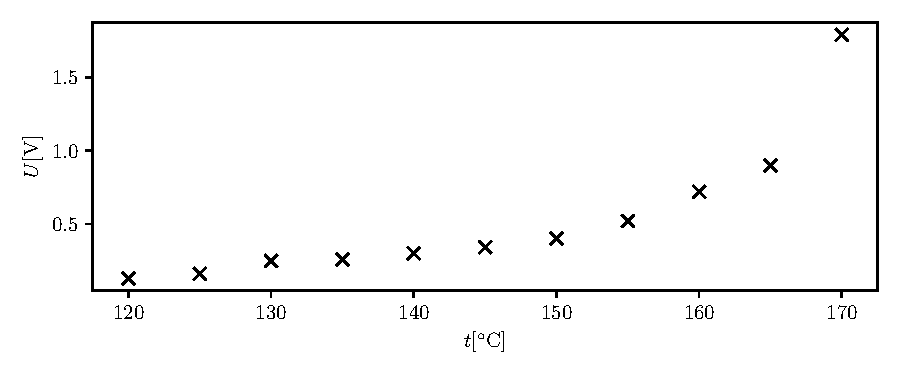
\includegraphics{heating.pdf}
    \vspace{0pt}
    \caption{Závislost odezvy detektoru na teplotě v pícce}
    \label{fig:heating}
\end{figure}


    Pomocí přepínání polarity proudu tekoucího magnetickým analyzátorem za postupného snižování jeho hodnoty jsme demagnetizovali jádro analyzátoru.
    Poté jsme programem Stern-Gerlach proměřili závislost odezvy detektoru (závisející na počtu dopadajících atomů) na poloze detektoru pro různé hodnoty proudu protékajícího magnetickým analyzátorem a odpovídající hodnoty gradientu magnetického pole.
    Okometricky jsme odhadnuli polohy maxim píků a určili jejich vzdálenosti.
    Naměřené hodnoty jsou shrnuty v tabulce~\ref{tab:spread} a v grafech na obrázku~\ref{fig:curves}.

    
\begin{table}[h]
    \centering
    \setlength{\tabcolsep}{15pt}
    \begin{tabular}[t]{
  S[table-format=1.2]
  S[table-format=1.2]
  S[table-format=1.2]
  S[table-format=1.2]
  S[table-format=1.3]
} \toprule
{$I$} & {$B$} & {$\Delta x$} & {$q$}  & {$\frac{\partial B}{\partial x}$} \\
{[A]} & {[T]} & {[mm]}       & {[mm]} & {$[\si{\tesla\per\milli\metre}]$} \\ \midrule
 0.26 &  0.18 &         1.55 &   1.62 &                             0.070 \\
 0.38 &  0.28 &         1.89 &   2.25 &                             0.108 \\
 0.51 &  0.39 &         2.31 &   2.99 &                             0.151 \\
 0.77 &  0.57 &         3.14 &   4.36 &                             0.221 \\
 0.98 &  0.67 &         3.73 &   5.30 &                             0.259 \\ \bottomrule
\end{tabular}
    \vspace{0pt}
    \caption{Naměřené hodnoty vzdálenosti maxim píků závislostí na poli v analyzátoru}
    \label{tab:spread}
\end{table}

    
\begin{figure}[h!]
    \centering
    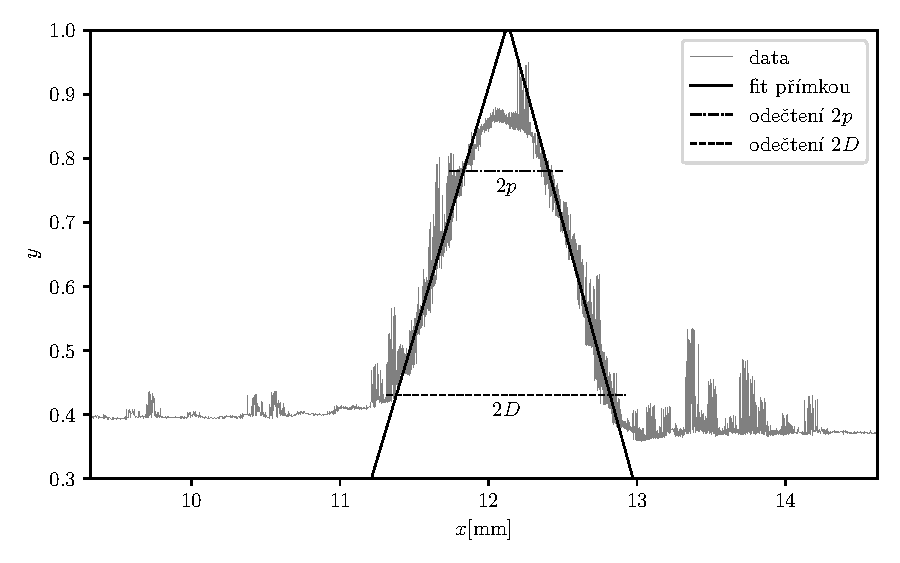
\includegraphics{0A_fit.pdf}
    \vspace{0pt}
    \caption{Závislost odezvy detektoru na jeho poloze pro nulové pole v analyzátoru}
    \label{fig:0A_fit}
\end{figure}

    
\begin{figure}[h!]
    \centering
    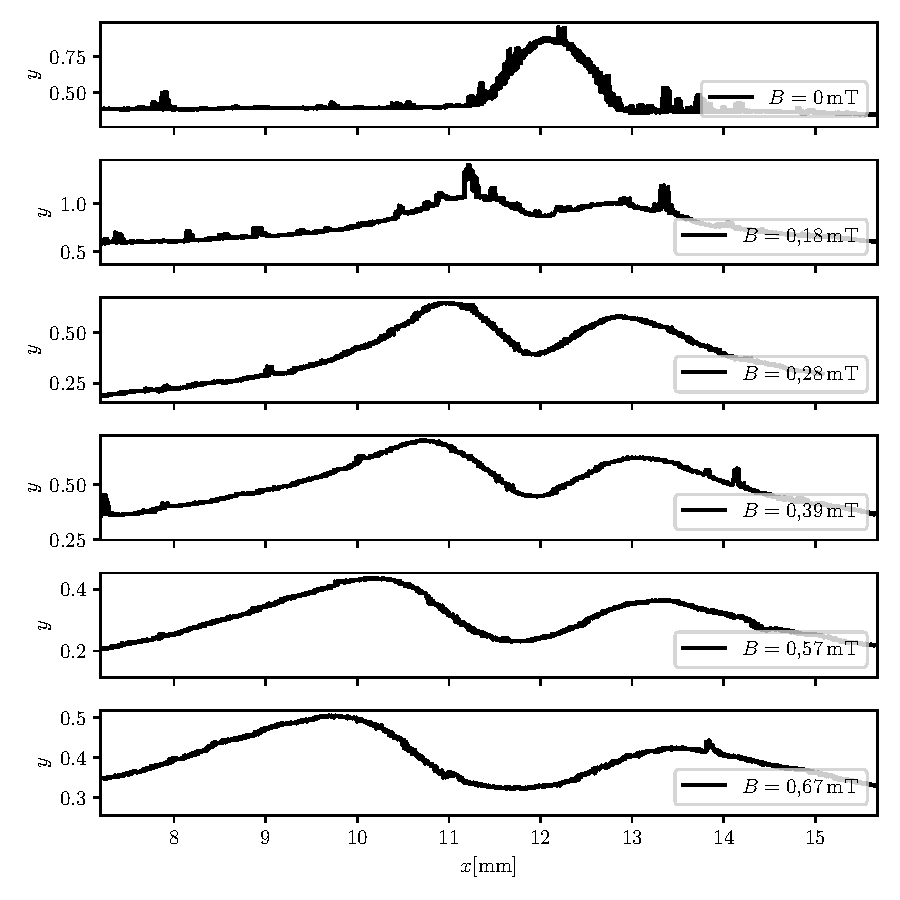
\includegraphics{curves.pdf}
    \vspace{0pt}
    \caption{Závislosti odezvy detektoru na jeho poloze pro různá pole v analyzátoru}
    \label{fig:curves}
\end{figure}


    Abychom mohli dopočítat hodnotu Bohrova magnetonu, určili jsme hodnotu výrazu $\frac{q}{\frac{\partial B}{\partial x}}$ pomocí lineární regrese zobrazené v grafu na obrázku~\ref{fig:spread}.
    Směrnice fitovací přímky je $ k = \SI{0.0493 \pm 0.0008}{\tesla\per\square\milli\metre} $.
    Pomocí vztahu~\eqref{eq:bohr} spočítáme hodnotu Bohrova magnetonu
    \[ \mu_B = \SI{1.30 \pm 0.04 e-23}{\joule\per\tesla}. \]

    Tabulková hodnota činí \[ \mu_{B, \text{tab}} = \SI{0.93 e-23}{\joule\per\tesla}. \]
    
\begin{figure}[h!]
    \centering
    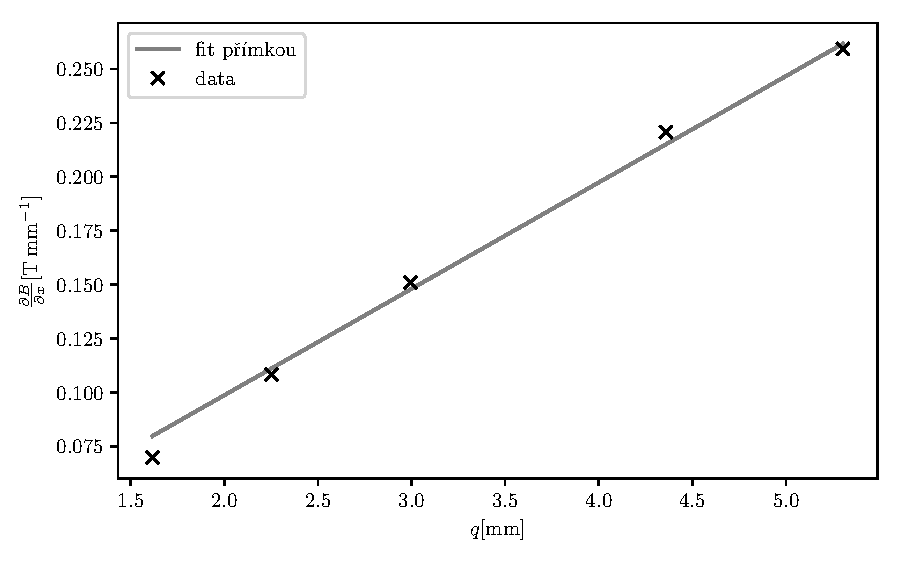
\includegraphics{spread.pdf}
    \vspace{0pt}
    \caption{Lineární fit pro výpočet Bohrova magnetonu}
    \label{fig:spread}
\end{figure}


    \section*{Diskuse}

    V tomto praktiku v podstatě nemáme kontrolu nad aparaturou a mnoho hodnot máme zadané a musíme jim věřit (délky aparatury, převodní vztahy atd.).
    Proto je poměrně obtížné určit zdroje chyb.
    Během praktika nebyla brána velká zřetel na chybovost měřicích přístrojů, jelikož největším zdrojem nepřesnosti byl okometrický odhad poloh maxim píků závislostí jakožto i (taktéž okometrický) odhad vhodných zón pro lineární regresi závislosti měřené bez přítomnosti pole v analyzátoru.

    Je zřejmé, že námi vypočtená hodnota Bohrova magnetonu výrazně nadhodnocuje tabulkovou hodnotu.

    \section*{Závěr}

    Po kontrole vakua v aparatuře a zprovoznění zdroje atomů a detektoru byly proměřeny závislosti odezvy detektoru na množství dopadajících atomů na poloze detektoru.
    Z těchto hodnot jsme získali hodnotu Bohrova magnetonu
    \[ \mu_B = \SI{1.30 \pm 0.04 e-23}{\joule\per\tesla}, \]
    která však nad rámec chyby nadhodnocuje tabulkovou hodnotu.

    \begin{thebibliography}{}

        \bibitem{pokyny}
        Pokyny k měření ``Prostorové kvantování magnetického momentu atomu (Sternův-Gerlachův experiment)'', dostupné z\\ \url{https://physics.mff.cuni.cz/vyuka/zfp/_media/zadani/texty/txt_411.pdf}, 27.\,11.\,2019

    \end{thebibliography}

\end{document}